 \chapter{О том, как Куба подружилась с СССР }


Если спросить в западных интернетах: “кто такой Фидель Кастро?”, общий ответ будет примерно таким: тиран и деспот, скрытый марксист, ложью и манипуляциями узурпировавший власть на когда-то столь славном Острове Свободы и сбросивший страну в коммунистическую бездну! В зависимости от ваших взглядов, это – либо сущая правда, либо вопиющая ложь, но вот что интересно: скрытый марксист? Неужели Кастро с самого начала планировал попасть под уютное крыло СССР?

Нет, не планировал. Да и сам Нерушимый Союз не имел никакого отношения к кубинской революции. Но тогда как же Куба дошла до советских ракет? Давайте поговорим об этом.

Начнем с декабря 1958 г. На Кубе очень интересно: повстанцы активно наступают, режим Батисты доживает последние дни. А в Мексике представитель одной импортной компании из Коста-Рики обращается в посольство Чехословакии, чтобы обсудить поставки вооружения и обмундирования для повстанцев Кастро. Верные идеалам коммунизма (читай, не способные принимать самостоятельные решения), чехословаки запрашивают инструкции у Москвы — последняя осторожничает, но в конце декабря всё же соглашается. Что, правда, уже было неважно, потому что через несколько дней режим Батисты пал, и необходимость в советской помощи отпала. Появились проблемы посложнее.

\begin{figure}[h!tb] 
	\centering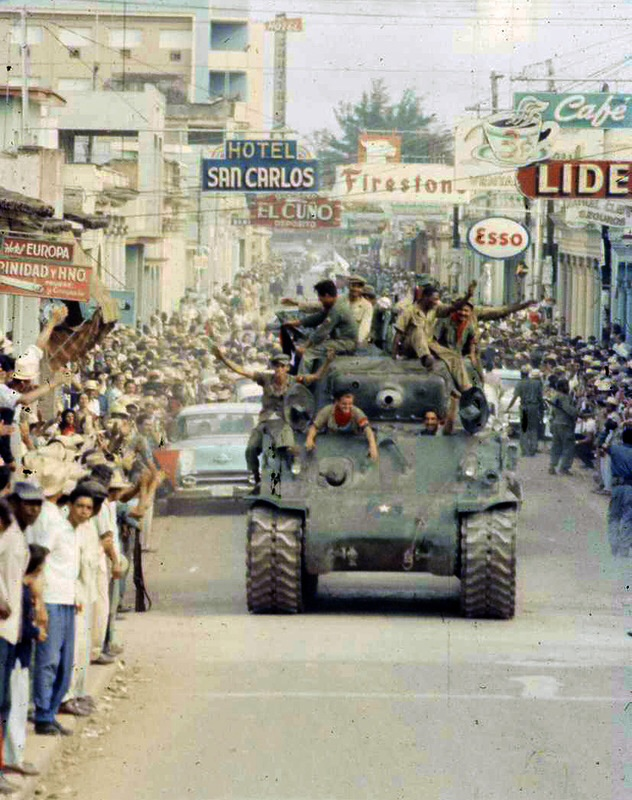
\includegraphics[scale=0.4]{KubaUSSR/jaXlM1B_0-U.jpg}
	%	\label{fig:scipion} % Unique label used for referencing the figure in-text\end{document}
	%	%\addcontentsline{toc}{figure}{Figure \ref{fig:placeholder}} % Uncomment to add the figure to the table of contents%----------------------------------------------------------------------------------------
	\caption{Гавана, 1959 }%	CHAPTER 2
\end{figure}

Деспот или освободитель, кем точно Фидель не был – так это дураком. И он прекрасно понимал, что стоит Кубе подать признаки уклона в социализм, как большой сосед дядя Сэм быстренько вмешается и наведёт порядок. Но революция только что свершилась, толкаются речи о третьем, независимом пути, влетать под крыло товарища Ивана как-то не хочется, а так как Батиста забрал с собой приличную часть золотовалютного запаса страны, то революции очень нужны деньги. Поэтому Фидель организует так называемую операцию «Правда» — информационную кампанию по укреплению имиджа Кубы в глазах американцев. Сначала организовываются публичные суды над пособниками Батисты, на которые приглашают иностранных журналистов, а затем, в апреле, сам Кастро отправляется в США, чтобы собрать плюсиков к пиару, а главное — выиграть для Кубы «план Маршалла». В ходе поездки он даже заявил, что американская собственность на Кубе останется неприкосновенной, что Куба не будет заигрывать с Советами, и что больше никакой диктатуры — ни личной, ни классовой — не будет.

\begin{figure}[h!tb] 
	\centering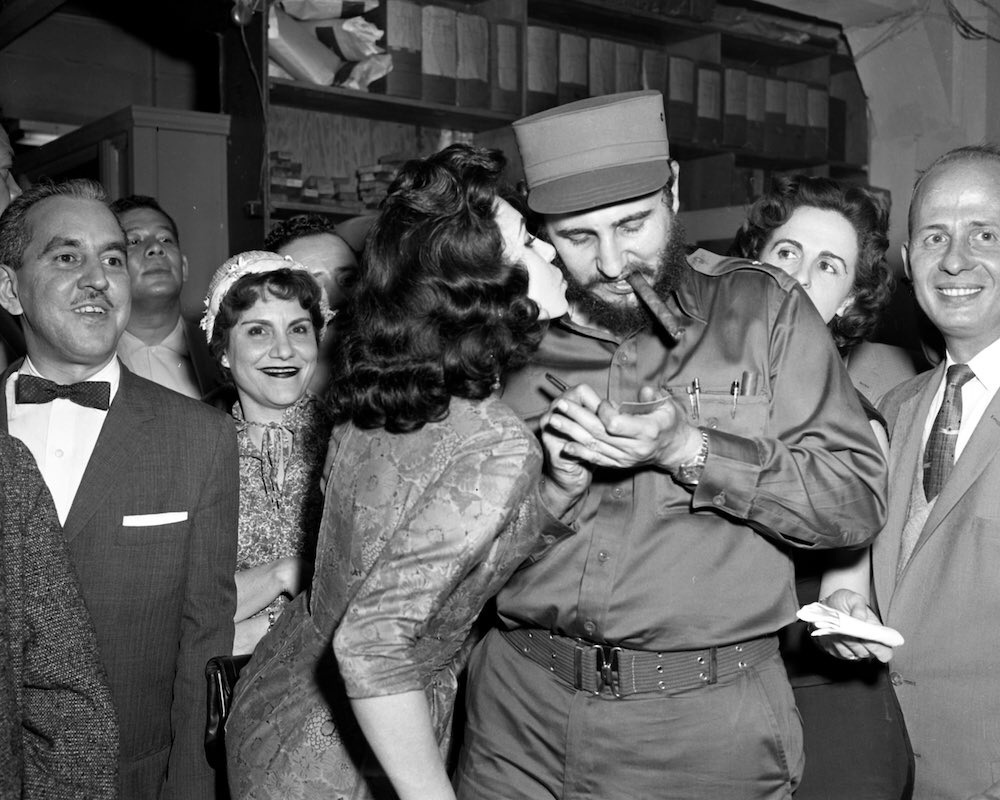
\includegraphics[scale=0.4]{KubaUSSR/9fJrgUUsNtI.jpg}
	%	\label{fig:scipion} % Unique label used for referencing the figure in-text\end{document}
	%	%\addcontentsline{toc}{figure}{Figure \ref{fig:placeholder}} % Uncomment to add the figure to the table of contents%----------------------------------------------------------------------------------------
	\caption{Фидель в Нью-Йорке, апрель 1959. Да, американская верхушка приняла Кастро прохладно — а вот публика была в полном восторге! }%	CHAPTER 2
\end{figure}

И пока Фидель выступал в США, а публика сходила с ума от обожания, Куба таки начинала заигрывать с Советами. А точнее, заигрывать начал брат Фиделя, Рауль. Тайный член Национально-социалистической партии (НСП), министр Революционных вооруженных сил Кубы, Кастро-младший, в отсутствие старшего, послал своего представителя прямиком в Москву, чтобы договориться об отправке нескольких военных советников (выходцев из испанской компартии) для помощи Кубинской армии. Москва согласилась, даже оплатила отправку, а заодно помогла с поставкой сельхозтехники и закупкой кубинского сахара, но это было всё, на что Кремль в тот момент был готов. Не хотелось Союзу злить Америку на её же заднем дворе.

\begin{figure}[h!tb] 
	\centering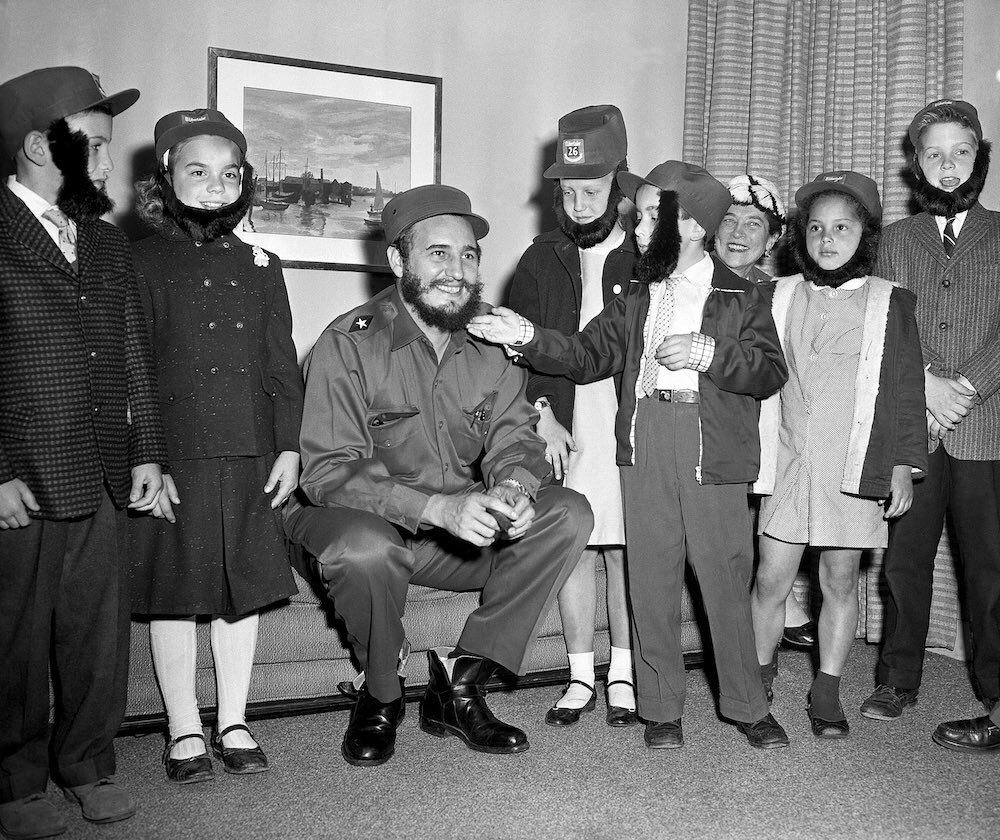
\includegraphics[scale=0.4]{KubaUSSR/hHtSL7ehizk.jpg}
	%	\label{fig:scipion} % Unique label used for referencing the figure in-text\end{document}
	%	%\addcontentsline{toc}{figure}{Figure \ref{fig:placeholder}} % Uncomment to add the figure to the table of contents%----------------------------------------------------------------------------------------
	\caption{Фидель и дети. Интересно, попадут ли в будущем эти мальчишки во Вьетнам?! }%	CHAPTER 2
\end{figure}

Но вариантов у Кастро уже особо и не оставалось. Поездка в США не сильно помогла: президент Эйзенхауэр отказал во встрече, сославшись на занятость («Он предпочел партию в гольф встрече с руководителем самой выдающейся революции в Западном полушарии»), а остальные представители американской верхушки встретили Фиделя довольно прохладно, без энтузиазма. Да, студенты Гарварда, в котором Фидель пламенно выступил, остались в экстазе, но ведь не студенты будут спонсировать кубинскую экономику. Поэтому из штатов Фидель вернулся без денег и почти сразу же национализировал кучу американских телефонных, электрических, нефтеперегонных компаний и 36 сахарных заводов. В ответ США прекратили импорт сахара и экспорт нефтепродуктов. Дядя Сэм всё же обиделся.

Прыгнем на пару месяцев вперед, в сентябрь. Пока Хрущев в США смотрит на панталоны Ширли Маклейн, кубинцы обращаются к Польше с просьбой о поставках оружия. Не менее верная идеалам коммунизма Варшава запрашивает инструкции у Москвы. Президиум ЦК, в отсутствие Хрущева, принимается активно обсуждать запрос, и общее настроение как-то не в пользу Кубы. К тому моменту уже произошла встреча Хрущева и Эйзенхауэра в Кемп-Дэвиде, символизировавшая разрядку в отношениях СССР и США, и помощь Кубе могла разрушить «дух Кэмп-Дэвида». К счастью для Кубы, Хрущев вернулся раньше, чем было принято решение. Уязвленный экономическим превосходством США, Хрущев решил оказать военную помощь Кубе.

Да, просто решил оказать. Повертев на детородном органе мнение Президиума ЦК, МИДа, международного отдела ЦК КПСС. Даже Сталин в свое время не решался лезть в дела Латинской Америки, а Никита решился. Через пять лет, когда на детородном органе повертят самого Хрущева, об этом решении вспомнят, как об ошибочном.

\begin{figure}[h!tb] 
	\centering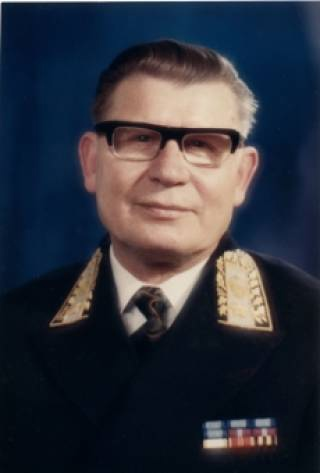
\includegraphics[scale=0.4]{KubaUSSR/4zrs8J7BhV4.jpg}
	%	\label{fig:scipion} % Unique label used for referencing the figure in-text\end{document}
	%	%\addcontentsline{toc}{figure}{Figure \ref{fig:placeholder}} % Uncomment to add the figure to the table of contents%----------------------------------------------------------------------------------------
	\caption{Павел Шитов, aka Александр Алексеев. Как гласит легенда, после шутки про буржуев от Кастро, Шитов перестал носить галстуки. }%	CHAPTER 2
\end{figure}

Но это будет через пять лет, а пока что Москва отправляет на Кубу представителя. 1 октября в Гавану прибывает сотрудник КГБ Павел Шитов... Ах нет, это прибыл советник посольства по вопросам культуры Александр Алексеев. Он практически сразу вышел на НСП, но, погуляв по Гаване и ощутив слегка когнитивный диссонанс от кубинских газет, в которых антиамериканские лозунги соседствовали с яркой антисоветской риторикой, здраво решил, что за кубинскую революцию ему пояснить может только Фидель, и ни кто иной. Поэтому Алексеев сначала вышел на Че Гевару, а затем добился личной встречи с Кастро. Встреча, конечно, была странная: прилично одетый Алексеев, в темном костюме и сером галстуке, увидел перед собой двух хорошо вооруженных бородачей — самого Фиделя и его помощника. Кастро, разумеется, не упустил возможность посмеяться:

— Александре, сколько лет Вашей революции?
— 42 года.
— Значит, через 42 года мы тоже превратимся в буржуев.

Но несмотря на это, встреча прошла успешно: через Алексеева братья Кастро получили выход прямо на Москву, и на Кубу пошли первые оружейные поставки. Сначала, правда, только старое вооружение времен Второй Мировой, чтобы не злить сильно американцев, если они как-то прознают. Но этого было достаточно, чтобы общественное мнение на Кубе начало смещаться в сторону СССР. Например, Че, который изначально негативно относился к идее сближения с любой из сверхдержав, в итоге согласился с курсом на Союз. И, конечно же, чем дальше «левела» Куба, тем больше злилась Америка. Но это уже другая история.

Могла ли Куба обойтись без помощи? Вряд ли. Страна после революции столкнулась с тяжелым финансовым положением, и как бы того ни хотели кубинские газеты, в условиях Кубы нельзя было и рыбку съесть, и на экономическую помощь получить. Кастро верно попытался сначала получить рыбку от США, тем более что он сам до этого благосклонно относился к Америке, но, судя по всему, в США его просто не поняли — они видели левого революционера-смутьяна, который зачем-то пришел к ним за деньгами, и попросту не придали ему должного значения. Поэтому выхода особо не оставалось, кроме как национализировать американскую собственность и пойти на сближение с советским блоком.

Ну а то, что будет дальше — и «Залив Свиней», и «Анадырь», и вот это вот все — мы с вами обсудим потом.



Автор Алексей Иванов.  Оригинал \url{https://vk.com/wall-162479647_287551}

\#Иванов@catx2
\#Заметка@catx2


